%!TEX encoding = UTF-8 Unicode
\documentclass[a4paper,11pt]{article}

	\usepackage[utf8]{inputenc}
	\usepackage[italian]{babel}
	\usepackage{hyperref}	%Consente l'inserimento di \url
	\usepackage{booktabs}	%Utilità di abbellimento tabelle
	\usepackage{longtable}
	\usepackage{tabularx}
	%\usepackage{widetable}
	\usepackage{array}
	\usepackage{listings}
	\usepackage{graphicx}
	\usepackage{caption}
	\usepackage{fancyhdr}
	\newenvironment{fixpic}{}{} % [1]
	\usepackage[a4paper,top=3cm,bottom=3cm,left=2.5cm,right=2.5cm]{geometry}
	%******
	\usepackage{makeidx}
	\usepackage{textcomp}
	\usepackage{multirow}
	\usepackage{rotfloat}
	\usepackage{lastpage}
	\usepackage{array}
	\usepackage{float}
	% *************************************
	% QUI CODICE PER \SUBSUBSUBSECTION
	\usepackage{titlesec}
	\titleclass{\subsubsubsection}{straight}[\subsection]
	
	\newcounter{subsubsubsection}[subsubsection]
	\renewcommand\thesubsubsubsection{\thesubsubsection.\arabic{subsubsubsection}}
	\renewcommand\theparagraph{\thesubsubsubsection.\arabic{paragraph}} % optional; useful if paragraphs are to be numbered
	
	\titleformat{\subsubsubsection}
	  {\normalfont\normalsize\bfseries}{\thesubsubsubsection}{1em}{}
	\titlespacing*{\subsubsubsection}
	{0pt}{3.25ex plus 1ex minus .2ex}{1.5ex plus .2ex}
	
	\makeatletter
	\renewcommand\paragraph{\@startsection{paragraph}{5}{\z@}%
	  {3.25ex \@plus1ex \@minus.2ex}%
	  {-1em}%
	  {\normalfont\normalsize\bfseries}}
	\renewcommand\subparagraph{\@startsection{subparagraph}{6}{\parindent}%
	  {3.25ex \@plus1ex \@minus .2ex}%
	  {-1em}%
	  {\normalfont\normalsize\bfseries}}
	\def\toclevel@subsubsubsection{4}
	\def\toclevel@paragraph{5}
	\def\toclevel@paragraph{6}
	\def\l@subsubsubsection{\@dottedtocline{4}{7em}{4em}}
	\def\l@paragraph{\@dottedtocline{5}{10em}{5em}}
	\def\l@subparagraph{\@dottedtocline{6}{14em}{6em}}
	\makeatother
	
	\setcounter{secnumdepth}{4}
	\setcounter{tocdepth}{4}
	%FINE \SUBSUBSUBSECTION
	%****************************************
	%STYLE PER INSERIMENTO DEL CODICE
	\lstdefinestyle{style1}{
	  belowcaptionskip=1\baselineskip,
	  breaklines=true,
	  frame=L,
	  xleftmargin=\parindent,
	  language=Pascal,
	  showstringspaces=false,
	  basicstyle=\footnotesize\ttfamily,
	  keywordstyle=\bfseries\color{blue},
	  commentstyle=\itshape\color{blue},
	  identifierstyle=\color{blue},
	  stringstyle=\color{orange},
	}
	
	\lstdefinestyle{style2}{
	  belowcaptionskip=1\baselineskip,
	  frame=L,
	  xleftmargin=\parindent,
	  language=C,
	  basicstyle=\footnotesize\ttfamily,
	  commentstyle=\itshape\color{blue},
	}
	\lstset{style=style1}
	
	%FINE STYLE INSERIMENTO CODICE
	%*****************************************
	\usepackage[default]{cantarell} %% Use option "defaultsans" to use cantarell as sans serif only
	\usepackage[T1]{fontenc}        %% for font
	\hypersetup{colorlinks, linkcolor=black, urlcolor=blue}
	\newcommand{\addglos}{\begin{scriptsize}{\textbf{\ped{G}}} \end{scriptsize}} 
	\pagestyle{fancy}
	\fancyhead{}
	\fancyfoot{}
	%\fancyhead[L]{
\includegraphics[scale=0.28]{team_not_found.jpeg}}
	\fancyhead[L]{
\includegraphics[scale=0.15]{../../team404_small.jpg} \hspace{2mm} QUIZZIPEDIA}
	\fancyhead[R]{\leftmark}
	\fancyfoot[L]{Universit\`a degli studi di Padova - IS 2015/2016 \\ \url{team404swe@gmail.com}}

	
	%Commando usato per la tabella di informazioni sul documento
	\newcommand{\introtab}[9]{
		\begin{table}[ht]
		\begin{center}		
		\begin{tabular}{r l}			
			\toprule		
			\multicolumn{2}{c}{\textbf{ Informazioni sul documento }} \\
			\midrule 
			\textbf{Nome Documento}			& \vline \hspace{3.5 mm} {#1} \\
			\textbf{Versione}				& \vline \hspace{3.5 mm} {#2} \\
			\textbf{Uso} 					& \vline \hspace{3.5 mm} {#3} \\
			\textbf{Data Creazione} 		& \vline \hspace{3.5 mm} {#4} \\
			\textbf{Data Ultima Modifica} 	& \vline \hspace{3.5 mm} {#5} \\
			\textbf{Redazione}				& \vline \hspace{3.5 mm} {#6} \\
											%& \vline \hspace{3.5 mm} {#7} \\	
			\textbf{Verifica} 				& \vline \hspace{3.5 mm} {#7}	\\
			\textbf{Approvazione}			& \vline \hspace{3.5 mm} {#8}\\	
			\textbf{Committente} 			& \vline \hspace{3.5 mm} Zucchetti SPA\\
			\textbf{Lista di distribuzione} & \vline \hspace{3.5 mm} Prof. Vardanega Tullio \\														& \vline \hspace{3.5 mm} TEAM404 \\
	\bottomrule	
	\end{tabular}
	\end{center}
	\end{table}
	}
	% Comando di inizio del registro
	\newcommand{\beginregistro}{
		%\begin{longtable}{{|p{0.10\textwidth}|p{0.20\textwidth}|p{0.15\textwidth}|p{0.50\textwidth}|}}
		\begin{longtable}{{|p{1.5cm}|p{2.5cm}|p{2cm}|p{8cm}|}} 
	 		\hline	
	}
	% commando usato pr inserire una riga al registro delle modifiche
	\newcommand{\rigaregistro}[4]{
		{\footnotesize #1} & {\footnotesize #2} &  {\footnotesize #3} &  {\footnotesize #4} \\
			\hline	
	}
	% Comando di fine registro
	\newcommand{\fineregistro}{ \end{longtable}	}
	
	%************************************************
	% commandi per il GLOSSARIO
	%***********************************************
	% Commando di inizio tabella Glossario
	\newcommand{\beginglos}{
		\begin{longtable}{{p{0.20\textwidth}p{0.65\textwidth}}}	
	}
	% Commando per i termini del glossario
	
	\newcommand{\itemglos}[2]{
		\textbf{#1 :} & {#2} \\ \\ \\
	}
	% Commando fine Glossario
	\newcommand{\fineglos}{ \end{longtable} }
	% Comando per aggiungere una ssezione numerata con lettere al glossario
	\newcommand{\sezione}{
	\subsection{}	
	\rule[0.3pt]{\linewidth}{0.4pt} \\ % Linea orizzontale
	}
	
\newcommand{\sezioneglos}[1] { 
  \newpage
  \cleardoublepage
  \phantomsection
  \addcontentsline{toc}{section}{#1}
  \vspace{11pt}
  \textbf{\huge{#1} } % Lettera grande 
  \\
  \rule[0.3pt]{\linewidth}{0.4pt} \\ % Linea orizzontale
  \fancyhead[R]{#1}
}

\newcommand*{\thead}[1]{\multicolumn{1}{c}{\bfseries #1}}

\makeindex
	\title{\textbf{{\fontsize{8mm}{5mm}\selectfont QUIZZIPEDIA}}}
	\date{}
	\author{}

\begin{document}
\pagenumbering{Roman}
	\maketitle
	\thispagestyle{empty}
	\begin{center}
	
\includegraphics{team_not_found.jpg}\\
	\fontsize{5mm}{3mm}\url{team404swe@gmail.com}\\
	
	\vspace{50mm}
	\textbf{Analisi dei Requisiti 1.0}
	%\'end{center}
	%\'begin{center}
	%\vspace{4mm}
	\end{center}
	
	%qui
	\introtab{Analisi dei Requisiti}		%1 nome documento
			{1.0} 							%2 versione
			{Esterno} 						%3 Uso
			{20 dicembre 2015} 				%4 Data creazione
			{\today} 						%5 Data mod
			{A. Beccaro - L. Alessio - M.Crivellaro}	%6 Redazione
			{Andrea Multineddu} 				%7 Verifica
			{Davide Bortot} 		%8 Approvazione
	%qui
	\newpage
	\thispagestyle{empty}
	\null
	\newpage
		
	\hspace{30 mm}
	\fancyhead[R]{REGISTRO DELLE MODIFICHE}
	\fancyfoot[R]{\thepage}
	\section*{Registro delle modifiche}
	
		\beginregistro
			\rigaregistro{\textbf{Versione}}{\textbf{Autore}}{\textbf{Data}}{\hspace{5 mm} \textbf{Descrizione}}
	 		\rigaregistro{1.0.1}{Alex Beccaro (Analista)}{28/04/2016}{Ampliamento contesto d'uso. Correzione e ampliamento casi d'uso.}
			\rigaregistro{1.0}{Davide Bortot (Responsabile)}{16/03/2016}{Approvazione del documento.}
			\rigaregistro{0.3}{Andrea Multineddu (Verificatore)}{15/03/2016}{Revisione del documento completo.}
			\rigaregistro{0.2.3}{Alex Beccaro (Analista)}{15/03/2016}{Controllo generale.}
			\rigaregistro{0.2.2}{Martin Mbouenda (Amministratore)}{14/03/2016}{Modificata struttura del documento per rispettare il nuovo template.}	
	 		\rigaregistro{0.2.1}{Martin Mbouenda (Amministratore)}{10/03/2016}{Segnalata incongruenza col nuovo template dei documenti.}	 		
	 		\rigaregistro{0.2}{Andrea Multineddu (Verificatore)}{22/01/2016}{Prima revisione del documento.}	 		
	 		\rigaregistro{0.1.3}{Alex Beccaro (Analista)}{21/01/2016}{Redazione mappatura dei requisiti e dei casi d'uso.}
	 		\rigaregistro{0.1.2}{Marco Crivellaro (Analista)}{19/01/2016}{Modifica e completamento della sezione dei requisiti.}
	 		\rigaregistro{0.1.1}{Alex Beccaro (Analista)}{18/01/2016}{Correzioni problemi trovati nell'ultima verifica. Redazione parziale dei requisiti}
	 		\rigaregistro{0.1.0}{Andrea Multineddu (Verificatore)}{15/01/2016}{Prima revisione del documento. Segnalati problemi da sistemare.}
	 		\rigaregistro{0.0.5}{Alex Beccaro (Analista)}{13/01/2016}{Controllo, correzione e completamento della sezione dei casi d'uso.}
	 		\rigaregistro{0.0.4}{Marco Crivellaro (Analista)}{9/01/2016}{Inserimento casi d'uso e descrizione parziale di questi.}
	 		\rigaregistro{0.0.3}{Alex Beccaro (Analista)}{23/12/2015}{Redazione paragrafo "Descrizione del problema".}
	 		\rigaregistro{0.0.2}{Luca Alessio (Analista)}{22/12/2015}{Redazione paragrafo "Introduzione".}
	 		\rigaregistro{0.0.1}{Alex Beccaro (Analista)}{20/12/2015}{Prima stesura del documento. Impostazione del documento e redazione sommario.}	 		
			\caption{Versionamento del documento} 
		\fineregistro
	\newpage
	\fancyhead[R]{\leftmark}
	\tableofcontents
	\newpage
	\listoffigures	
	\listoftables
	\newpage
	
	\renewcommand{\arraystretch}{2}
	\section*{Sommario}
	Questo documento descrive l’analisi dei requisiti derivati dallo studio del capitolato d’appalto \textbf{Quizzipedia} commissionato da \textbf{Zucchetti S.p.A.}.
	
	\newpage
	\pagenumbering{arabic}
	\section{Introduzione}
	\subsection{Scopo del Documento}
	Nelle sezioni successive del presente documento, dopo una rapida visione d'insieme del prodotto che il gruppo Team 404 si prefigge di sviluppare, verranno individuati e chiaramente definiti i requisiti che faranno da cardine alla piattaforma \textbf{Quizzipedia}.
	\subsection{Scopo del Prodotto}
	Il progetto \textbf{Quizzipedia} ha come obiettivo lo sviluppo di un sistema software basato su tecnologie Web (Javascript, Node.js, HTML5, CSS3) che permetta la creazione, gestione e fruizione di questionari. Il sistema dovrà quindi poter archiviare i questionari suddivisi per argomento, le cui domande dovranno essere raccolte attraverso uno specifico linguaggio di markup (Quiz Markup Language) d'ora in poi denominato QML. In un caso d'uso a titolo esemplificativo, un "esaminatore" dovrà poter costruire il proprio questionario scegliendo tra le domande archiviate, ed il questionario così composto sarà presentato e fruibile all' "esaminando", traducendo l'oggetto QML in una pagina HTML, tramite un'apposita interfaccia web. Il sistema presentato dovrà inoltre poter proporre questionari preconfezionati e valutare le risposte fornite dall'utente finale.
	\subsection{Glossario}
	Viene allegato un glossario nel file ``\textit{glossario\_1.0.pdf}'' nel quale viene data una definizione a tutti i termini che in questo documento appaiono sottolineati.
	\subsection{Riferimenti}
		\subsubsection{Normativi}
		\begin{itemize}
			\item Capitolato d'appalto Quizzipedia:\\
			\url{http://www.math.unipd.it/~tullio/IS-1/2015/Progetto/C5.pdf}
			\item Norme di Progetto: "\textit{norme\_di\_progetto\_1.0.pdf}"
		\end{itemize}
		\subsubsection{Informativi}
		\begin{itemize}
			\item Corso di Ingegneria del Software anno 2015/2016:\\
			\url{http://www.math.unipd.it/~tullio/IS-1/2015/}
			\item Regole del progetto didattico:\\
			\url{http://www.math.unipd.it/~tullio/IS-1/2015/Dispense/PD01.pdf}
			\url{http://www.math.unipd.it/~tullio/IS-1/2015/Progetto/}\\
			\url{http://www.math.unipd.it/~tullio/IS-1/2015/Progetto/PD01b.html}
		\end{itemize}
	\pagebreak

	\newpage	
	\section{Descrizione del Problema}
	\subsection{Contesto d'uso}
		Il capitolato Quizzipedia ha come scopo quello della realizzazione di una piattaforma web. L'utente che accede al sito di Quizzipedia avrà la possibilità di svolgere questionari su vari argomenti e (se autenticato) di crearne di propri utilizzando una sintassi apposita: QML. Il lato front-end verrà realizzato utilizzado HTML5, CSS e Javascript mentre il server verrà gestito attraverso l'impiego della tecnologia Nodejs.\\
		Il prodotto Quizzipedia è pensato per essere adatto a vari contesti, semplice ed intuitivo, fruibile da parte di qualsiasi fascia di utente, anche quelle un po' carenti di conoscenze informatiche. Quizzipedia è perciò atto a sopperire, il più possibile, alla necessità di tecnici informatici per la gestione di quiz, rendendo qualsiasi utente capace di costruire questionari e inserirci domande scelte appositamente
	\subsection{Funzioni del Prodotto}
		Quizzipedia permette essenzialmente la compilazione questionari preconfezionati su un argomento scelto. Inoltre il sistema valuta le risposte date e fornisce un responso.
	\subsection{Vincoli di Utilizzo}
		Per poter usufruire dell'applicazione Quizzipedia è necessario disporre di una connessione di
rete, un browser web compatibile con HTML5 CSS3 e Javascript attivato.
	
	\newpage
	\section{Casi d'uso}
\subsection{Attori}
Gli attori del sistema sono gli utenti, che possono essere di due tipologie: autenticati o non autenticati.\\ 
L'utente non autenticato rappresenta un utente che non ha effettuato l'accesso. Inizialmente ogni attore è in questo stato, tuttavia può diventare autenticato eseguendo la registrazione o, nel caso l'abbia già fatta precedentemente, accedendo con la procedura di login. Oltre a questo ha la possibilità di  sfogliare i questionari presenti per categoria e compilarli.\\
L'utente autenticato è un utente che ha effettuato l'accesso al sistema tramite il form di login. Può tornare allo stato di utente non autenticato effettuando il logout. Inoltre, oltre a sfogliare e compilare questionari, ha la capacità di poter creare nuove domande e nuovi questionari.\\

\begin{figure}[h!]
\centering
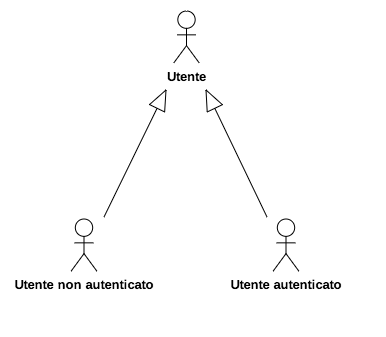
\includegraphics[scale=1]{../immagini/Actors.png}
\caption{Gerarchia attori}
\end{figure}

\newpage
\subsection{Sistema Quizzipedia}

\begin{figure}[h!]
\centering
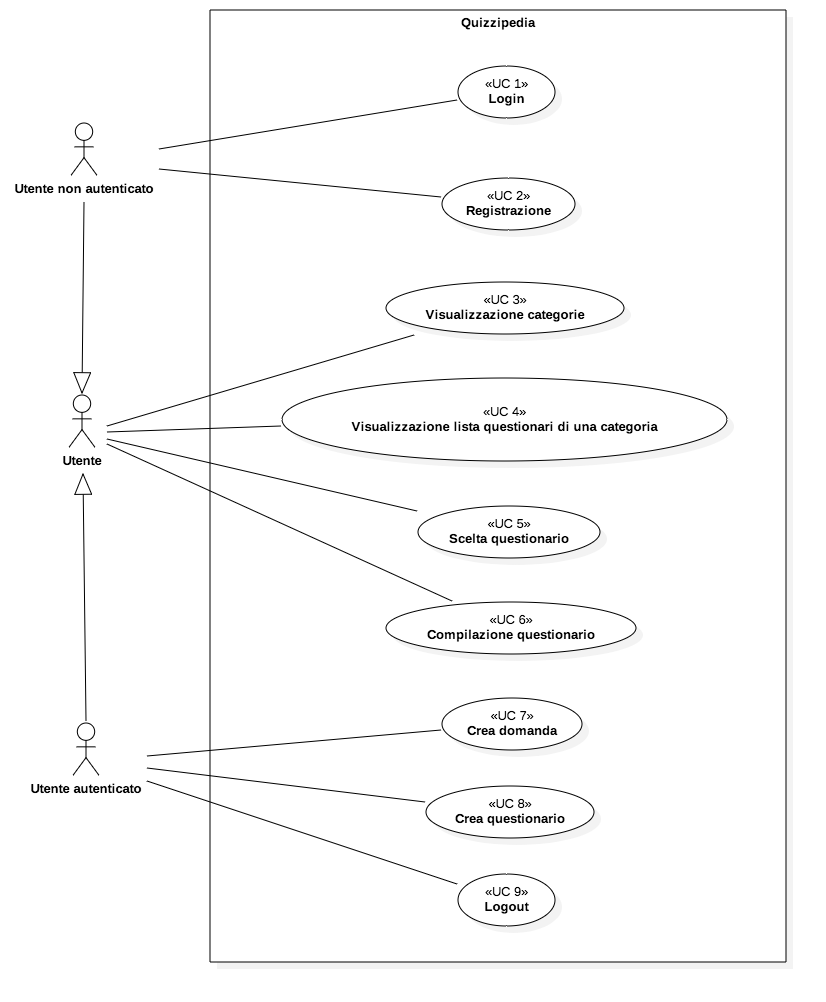
\includegraphics[scale=0.6]{../immagini/Main.png}
\caption{Sistema Quizzipedia}
\end{figure}
\ \\
\textbf{Attori:} \textit{utente non autenticato, utente autenticato}
\\ \\
\textbf{Descrizione:} caso d'uso generale che descrive le operazioni che i vari tipi di utenti possono effettuare all'interno del sistema.\\


\subsection{UC 1 - Login}

\begin{figure}[h!]
\centering
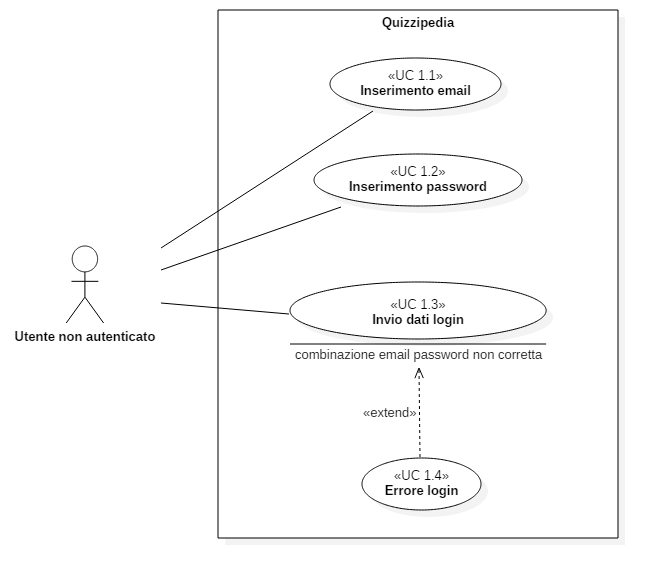
\includegraphics[scale=0.6]{../immagini/UC1.png}
\caption{Login}
\end{figure}
\ \\
\textbf{Attori:} \textit{utente non autenticato}
\\ \\
\textbf{Descrizione:} caso d'uso che descrive l'operazione di autenticazione al sistema. Comprende l'inserimento dei dati necessari, una procedura per il recupero della password e l'effettiva autenticazione.\\
\\
\textbf{Precondizioni:} il sistema può ricevere richieste di accesso da parte dell’utente non autenticato.\\
\\
\textbf{Postcondizioni:} l’utente che ora è autenticato.\\
\\
\textbf{Scenario:} l’utente inserisce i dati di accesso per effettuare il login al sistema (UC 1.1 e 1.2). Nel caso avesse dimenticato la password può accedere ad un form di recupero della stessa (UC 1.3). Se i dati inseriti sono corretti il sistema riconosce e autentica l'utente (UC 1.4) mentre se sono sbagliati viene visualizzato un messaggio di errore (UC 1.5).\\


\subsubsection{UC 1.1 - Inserimento email}

\textbf{Attori:} \textit{utente non autenticato}
\\ \\
\textbf{Descrizione:} caso d'uso che descrive l'inserimento della propria email da parte dell'utente.\\
\\
\textbf{Precondizioni:} il sistema permette l'inserimento di una email.\\
\\
\textbf{Postcondizioni:} l’utente ha inserito la propria email.\\
\\
\textbf{Scenario:} l’utente inserisce la propria email nell'apposito campo.\\


\subsubsection{UC 1.2 - Inserimento password}

\textbf{Attori:} \textit{utente non autenticato}
\\ \\
\textbf{Descrizione:} caso d'uso che descrive l'inserimento della propria password da parte dell'utente.\\
\\
\textbf{Precondizioni:} il sistema permette l'inserimento di una password.\\
\\
\textbf{Postcondizioni:} l’utente ha inserito la propria password.\\
\\
\textbf{Scenario:} l’utente inserisce la propria password nell'apposito campo.\\


\newpage
\subsubsection{UC 1.3 - Password dimenticata}

\begin{figure}[h!]
\centering
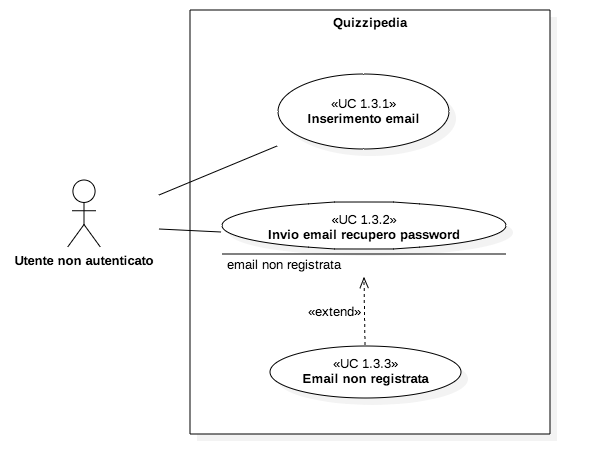
\includegraphics[scale=0.6]{../immagini/UC1_3.png}
\caption{Login}
\end{figure}
\ \\
\textbf{Attori:} \textit{utente non autenticato}
\\ \\
\textbf{Descrizione:} caso d'uso che descrive la procedura di recupero password in caso di dimenticanza.\\
\\
\textbf{Precondizioni:} l'utente non ricorda più la propria password.\\
\\
\textbf{Postcondizioni:} l’utente ha recuperato la propria password.\\
\\
\textbf{Scenario:} l’utente segue la procedura di recupero password e il sistema provvede a mandare una email con la password all'utente.\\


\subsubsubsection{UC 1.3.1 - Inserimento email}

\textbf{Attori:} \textit{utente non autenticato}
\\ \\
\textbf{Descrizione:} caso d'uso che descrive l'inserimento della email nella procedura di recupero password.\\
\\
\textbf{Precondizioni:} l'utente è nella procedura di recupero password.\\
\\
\textbf{Postcondizioni:} l’utente ha inserito la propria email.\\
\\
\textbf{Scenario:} l’utente inserisce la propria email nell'apposito campo.\\


\subsubsubsection{UC 1.3.2 - Invio email recupero password}

\textbf{Attori:} \textit{utente non autenticato}
\\ \\
\textbf{Descrizione:} caso d'uso che descrive l'invio al sistema della email nella procedura di recupero password.\\
\\
\textbf{Precondizioni:} l'utente ha inserito la propria email nella procedura di recupero password.\\
\\
\textbf{Postcondizioni:} l’utente riceve una email con la propria password dimenticata.\\
\\
\textbf{Scenario:} l’utente invia la propria email e il sistema manda una mail con la password dimenticata.\\
\\
\textbf{Extension points:} 
\begin{itemize}
	\item \textbf{Email non registrata:} La email inviata al sistema non corrisponde a nessun utente, viene visualizzato un messaggio di errore (UC 1.3.3)
\end{itemize}


\subsubsection{UC 1.4 - Invio dati login}

\textbf{Attori:} \textit{utente non autenticato}
\\ \\
\textbf{Descrizione:} caso d'uso che descrive l'autenticazione di un utente nel sistema.\\
\\
\textbf{Precondizioni:} l'utente ha inserito i propri dati e li ha inviati al sistema per l'autenticazione.\\
\\
\textbf{Postcondizioni:} l’utente è stato autenticato dal sistema.\\
\\
\textbf{Scenario:} l’utente invia i propri dati e il sistema lo autentica.\\
\\
\textbf{Extension points:} 
\begin{itemize}
	\item \textbf{Combinazione email password non corretta:} I dati inseriti e inviati al sistema non sono corretti, viene visualizzato un messaggio di errore (UC 1.5)
\end{itemize}


\newpage
\subsection{UC 2 - Registrazione}

\begin{figure}[h!]
\centering
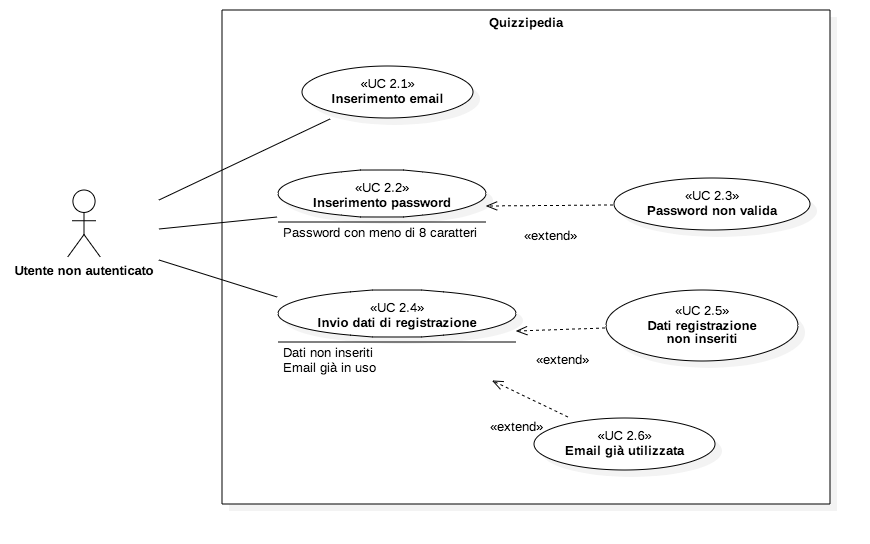
\includegraphics[scale=0.6]{../immagini/UC2.png}
\caption{Registrazione}
\end{figure}
\ \\
\textbf{Attori:} \textit{utente non autenticato}
\\ \\
\textbf{Descrizione:} caso d'uso che descrive l'operazione di registrazione al sistema. Comprende l'inserimento dei dati necessari, l'effettiva registrazione e l'autenticazione.\\
\\
\textbf{Precondizioni:} il sistema può registrare un nuovo utente.\\
\\
\textbf{Postcondizioni:} l’utente che ora è registrato e autenticato.\\
\\
\textbf{Scenario:} l’utente inserisce i dati di registrazione per effettuare il login al sistema (UC 2.1 e 2.2). Nel caso la password non abbia almeno 8 caratteri viene visualizzato un messaggio che avvisa l'utente che non è valida (UC 2.3). Se i dati inseriti sono corretti il sistema registra e autentica l'utente (UC 2.4). Se invece non sono stati inseriti alcuni campi viene visualizzato un messaggio di errore (UC 2.5). Nel caso in cui la email inserita sia già utilizzata da un altro utente viene visualizzato un messaggio di errore (UC 2.6).\\


\subsubsection{UC 2.1 - Inserimento email}

\textbf{Attori:} \textit{utente non autenticato}
\\ \\
\textbf{Descrizione:} caso d'uso che descrive l'inserimento della propria email da parte dell'utente.\\
\\
\textbf{Precondizioni:} il sistema permette l'inserimento di una email.\\
\\
\textbf{Postcondizioni:} l’utente ha inserito la propria email.\\
\\
\textbf{Scenario:} l’utente inserisce la propria email nell'apposito campo.\\


\subsubsection{UC 2.2 - Inserimento password}

\textbf{Attori:} \textit{utente non autenticato}
\\ \\
\textbf{Descrizione:} caso d'uso che descrive l'inserimento della propria password da parte dell'utente.\\
\\
\textbf{Precondizioni:} il sistema permette l'inserimento di una password.\\
\\
\textbf{Postcondizioni:} l’utente ha inserito la propria password.\\
\\
\textbf{Scenario:} l’utente inserisce la propria password nell'apposito campo.\\
\\
\textbf{Extension points:} 
\begin{itemize}
	\item \textbf{Password non valida:} La password non è valida in quanto è formata da meno di 8 caratteri, viene visualizzato un messaggio di errore (UC 2.3)
\end{itemize}


\subsubsection{UC 2.4 - Invio dati registrazione}

\textbf{Attori:} \textit{utente non autenticato}
\\ \\
\textbf{Descrizione:} caso d'uso che descrive la registrazione e l'autenticazione di un utente nel sistema.\\
\\
\textbf{Precondizioni:} l'utente ha inserito i propri dati e li ha inviati al sistema per la registrazione.\\
\\
\textbf{Postcondizioni:} l’utente è stato registrato e autenticato dal sistema.\\
\\
\textbf{Scenario:} l’utente invia i propri dati e il sistema lo registra come nuovo utente e lo autentica.\\
\\
\textbf{Extension points:} 
\begin{itemize}
	\item \textbf{Dati non inseriti:} alcuni dati richiesti non sono stati inseriti, viene visualizzato un messaggio di errore (UC 2.5)
	\item \textbf{Email già in uso:} l'email inserita è già stata registrata da un utente, viene visualizzato un messaggio di errore (UC 2.6)
\end{itemize}


\subsection{UC 3 - Visualizzazione categorie}

\begin{figure}[h!]
\centering
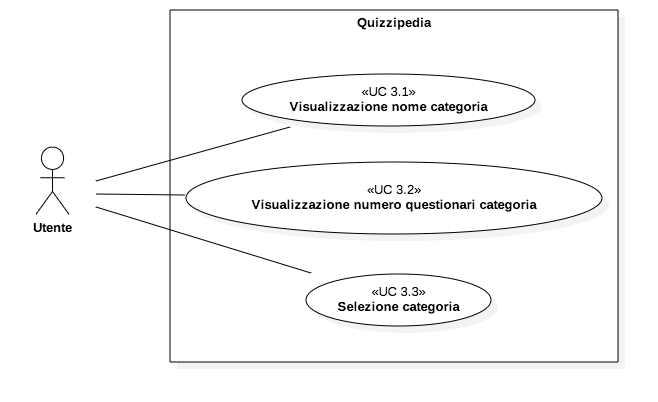
\includegraphics[scale=0.6]{../immagini/UC3.png}
\caption{Visualizzazione categorie}
\end{figure}
\ \\
\textbf{Attori:} \textit{utente}
\\ \\
\textbf{Descrizione:} caso d'uso che descrive la visualizzazione delle categorie di questionari. Per ogni categoria vengono visualizzati il nome e il numero di questionari relativi.\\
\\
\textbf{Precondizioni:} il sistema può accedere alla lista categorie.\\
\\
\textbf{Postcondizioni:} l’utente visualizza la lista delle categorie presenti.\\
\\
\textbf{Scenario:} l’utente accede alla sezione "Categorie". Per ogni categoria vengono visualizzati il nome (UC 3.1) e il numero di questionari relativi (UC 3.2).\\


\subsubsection{UC 3.1 - Visualizzazione nome categoria}

\textbf{Attori:} \textit{utente}
\\ \\
\textbf{Descrizione:} caso d'uso che descrive la visualizzazione dei nomi delle categorie.\\
\\
\textbf{Precondizioni:} L'utente è nella sezione "categorie".\\
\\
\textbf{Postcondizioni:} il sistema visualizza i nomi delle categorie.\\
\\
\textbf{Scenario:} l’utente visualizza i nomi delle categorie.\\


\subsubsection{UC 3.2 - Visualizzazione numero questionari categoria}

\textbf{Attori:} \textit{utente}
\\ \\
\textbf{Descrizione:} caso d'uso che descrive la visualizzazione del numero di questionari delle categorie.\\
\\
\textbf{Precondizioni:} L'utente è nella sezione "categorie".\\
\\
\textbf{Postcondizioni:} il sistema visualizza il numero di questionari delle categorie.\\
\\
\textbf{Scenario:} l’utente visualizza il numero di questionari delle categorie.\\


\subsection{UC 4 - Visualizzazione lista questionari categoria}

\begin{figure}[h!]
\centering
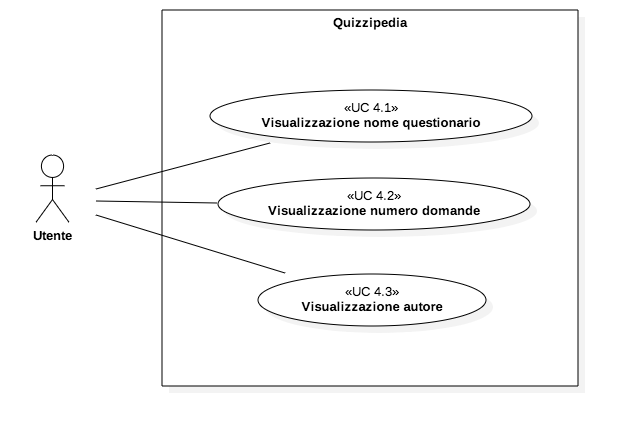
\includegraphics[scale=0.6]{../immagini/UC4.png}
\caption{Visualizzazione lista questionari categoria}
\end{figure}
\ \\
\textbf{Attori:} \textit{utente}
\\ \\
\textbf{Descrizione:} caso d'uso che descrive la visualizzazione della lista dei questionari di una categoria. Per ogni questionario vengono visualizzati il nome, il numero di domande e l'autore.\\
\\
\textbf{Precondizioni:} l'utente ha selezionato una categoria.\\
\\
\textbf{Postcondizioni:} l’utente visualizza la lista dei questionari della categoria selezionata.\\
\\
\textbf{Scenario:} l’utente seleziona una categoria e visualizza i questionari relativi. Per ogni questionario vengono visualizzati il nome (UC 4.1), il numero di domande (UC 4.2) e l'autore (UC 4.3).\\


\subsubsection{UC 4.1 - Visualizzazione nome questionario}

\textbf{Attori:} \textit{utente}
\\ \\
\textbf{Descrizione:} caso d'uso che descrive la visualizzazione dei nomi dei questionari.\\
\\
\textbf{Precondizioni:} L'utente visualizza la lista dei questionari della categoria selezionata.\\
\\
\textbf{Postcondizioni:} il sistema visualizza i nomi dei questionari.\\
\\
\textbf{Scenario:} l’utente visualizza i nomi dei questionari.\\


\subsubsection{UC 4.2 - Visualizzazione numero domande}

\textbf{Attori:} \textit{utente}
\\ \\
\textbf{Descrizione:} caso d'uso che descrive la visualizzazione del numero di domande dei questionari.\\
\\
\textbf{Precondizioni:} l'utente visualizza la lista dei questionari della categoria selezionata.\\
\\
\textbf{Postcondizioni:} il sistema visualizza il numero di domande dei questionari.\\
\\
\textbf{Scenario:} l’utente visualizza il numero di domande dei questionari.\\


\subsubsection{UC 4.3 - Visualizzazione autore}

\textbf{Attori:} \textit{utente}
\\ \\
\textbf{Descrizione:} caso d'uso che descrive la visualizzazione degli autori dei questionari.\\
\\
\textbf{Precondizioni:} l'utente visualizza la lista dei questionari della categoria selezionata.\\
\\
\textbf{Postcondizioni:} il sistema visualizza gli autori dei questionari.\\
\\
\textbf{Scenario:} l’utente visualizza gli autori dei questionari.\\


\subsection{UC 5 - Scelta questionario}

\textbf{Attori:} \textit{utente}
\\ \\
\textbf{Descrizione:} caso d'uso che descrive la scelta di un questionario.\\
\\
\textbf{Precondizioni:} il sistema permette la selezione di questionari.\\
\\
\textbf{Postcondizioni:} l’utente ha selezionato un questionario e può procedere con la compilazione.\\
\\
\textbf{Scenario:} l’utente seleziona un questionario. Il sistema entra in modalità compilazione del questionario.\\


\subsection{UC 6 - Compilazione questionario}

\begin{figure}[h!]
\centering
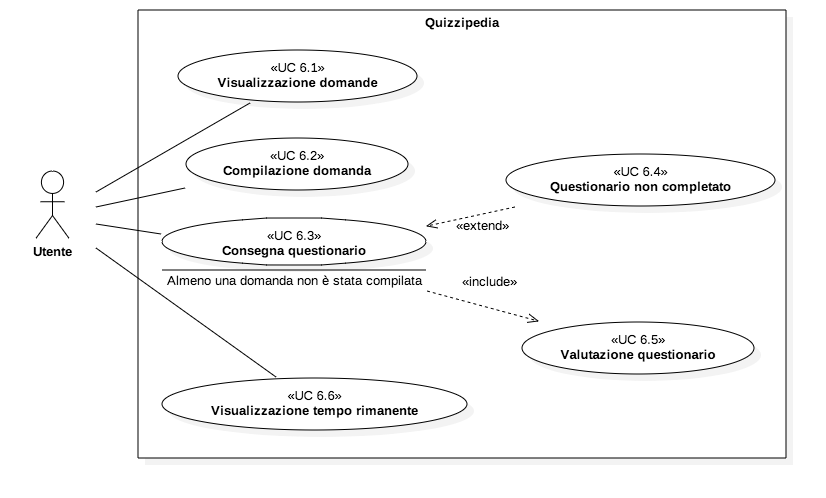
\includegraphics[scale=0.6]{../immagini/UC6.png}
\caption{Compilazione questionario}
\end{figure}
\ \\
\textbf{Attori:} \textit{utente}
\\ \\
\textbf{Descrizione:} caso d'uso che descrive la compilazione di un questionario. Comprende la visualizzazione e compilazione delle domande, la consegna e la valutazione del questionario.\\
\\
\textbf{Precondizioni:} l'utente può compilare un questionario.\\
\\
\textbf{Postcondizioni:} l’utente ha compilato un questionario e ne vede la valutazione.\\
\\
\textbf{Scenario:} l’utente compila il questionario. Questo comprende la compilazione delle domande (UC 6.2) e la consegna (UC 6.3). In caso alla consegna ci siano domande non compilate viene visualizzato un messaggio di errore (UC 6.4). Dopo la consegna avviene la valutazione del questionario e la visualizzazione dei risultati (UC 6.5).\\


\subsubsection{UC 6.1 - Visualizzazione domande}

\begin{figure}[h!]
\centering
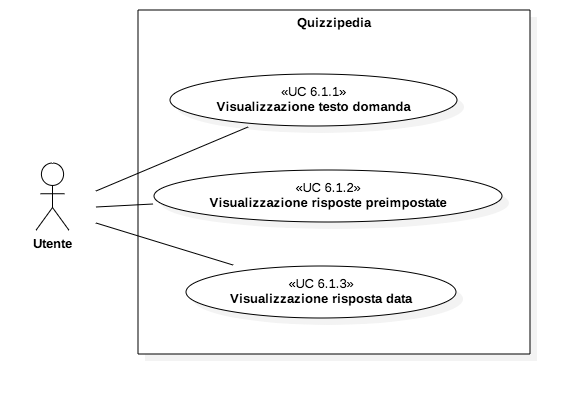
\includegraphics[scale=0.6]{../immagini/UC6_1.png}
\caption{Visualizzazione domande}
\end{figure}
\ \\
\textbf{Attori:} \textit{utente}
\\ \\
\textbf{Descrizione:} caso d'uso che descrive la visualizzazione delle domande di un questionario.\\
\\
\textbf{Precondizioni:} l'utente visualizza un questionario.\\
\\
\textbf{Postcondizioni:} il sistema visualizza le domande del questionario.\\
\\
\textbf{Scenario:} l’utente visualizza le domande del questionario.\\


\subsubsubsection{UC 6.1.1 - Visualizzazione testo domanda}

\textbf{Attori:} \textit{utente}
\\ \\
\textbf{Descrizione:} caso d'uso che descrive la visualizzazione del testo delle domande.\\
\\
\textbf{Precondizioni:} l'utente visualizza una lista di domande.\\
\\
\textbf{Postcondizioni:} il sistema visualizza il testo delle domande.\\
\\
\textbf{Scenario:} l’utente visualizza il testo delle domande.\\


\subsubsubsection{UC 6.1.2 - Visualizzazione risposte preimpostate}

\textbf{Attori:} \textit{utente}
\\ \\
\textbf{Descrizione:} caso d'uso che descrive la visualizzazione delle risposte preimpostate.\\
\\
\textbf{Precondizioni:} l'utente visualizza una domanda. La domanda ha delle risposte preimpostate.\\
\\
\textbf{Postcondizioni:} il sistema visualizza le risposte preimpostate.\\
\\
\textbf{Scenario:} l’utente visualizza le risposte preimpostate.\\


\subsubsubsection{UC 6.1.3 - Visualizzazione risposta data}

\textbf{Attori:} \textit{utente}
\\ \\
\textbf{Descrizione:} caso d'uso che descrive la visualizzazione della risposta data.\\
\\
\textbf{Precondizioni:} l'utente ha risposto ad una domanda.\\
\\
\textbf{Postcondizioni:} il sistema visualizza la risposta data.\\
\\
\textbf{Scenario:} l’utente visualizza la risposta data.\\


\subsubsection{UC 6.2 - Compilazione domanda}

\begin{figure}[h!]
\centering
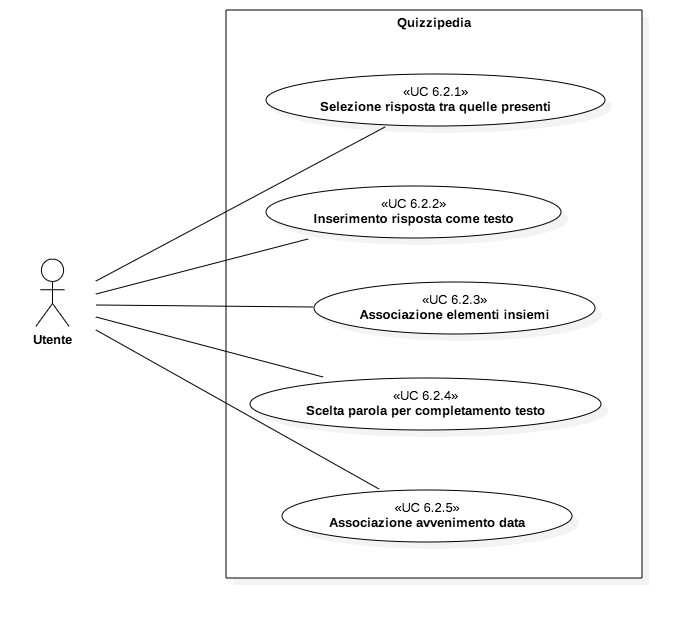
\includegraphics[scale=0.6]{../immagini/UC6_2.png}
\caption{Compilazione domanda}
\end{figure}
\ \\
\textbf{Attori:} \textit{utente}
\\ \\
\textbf{Descrizione:} caso d'uso che descrive la compilazione di una domanda.\\
\\
\textbf{Precondizioni:} l'utente visualizza una domanda.\\
\\
\textbf{Postcondizioni:} l'utente ha compilato una domanda.\\
\\
\textbf{Scenario:} l’utente visualizza una domanda e la compila.\\


\subsubsubsection{UC 6.2.1 - Selezione risposta tra le presenti}

\textbf{Attori:} \textit{utente}
\\ \\
\textbf{Descrizione:} caso d'uso che descrive la selezione di una delle risposte preimpostate.\\
\\
\textbf{Precondizioni:} l'utente visualizza una domanda con risposte preimpostate.\\
\\
\textbf{Postcondizioni:} l'utente ha selezionato una risposta.\\
\\
\textbf{Scenario:} l’utente seleziona una delle risposte preimpostate.\\


\subsubsubsection{UC 6.2.2 - Inserimento risposta come testo}

\textbf{Attori:} \textit{utente}
\\ \\
\textbf{Descrizione:} caso d'uso che descrive l'inserimento della risposta.\\
\\
\textbf{Precondizioni:} l'utente visualizza una domanda senza risposte preimpostate. Il sistema permette l'inserimento della risposta.\\
\\
\textbf{Postcondizioni:} l'utente ha inserito una risposta.\\
\\
\textbf{Scenario:} l’utente inserisce una risposta nel campo apposito.\\


\subsubsection{UC 6.3 - Consegna questionario}

\textbf{Attori:} \textit{utente}
\\ \\
\textbf{Descrizione:} caso d'uso che descrive la consegna di un questionario.\\
\\
\textbf{Precondizioni:} l'utente ha compilato un questionario.\\
\\
\textbf{Postcondizioni:} l’utente ha consegnato il questionario e ne ha ricevuto una valutazione.\\
\\
\textbf{Scenario:} l’utente consegna il questionario. Il sistema lo valuta e visualizza i risultati (UC 6.5).\\
\\
\textbf{Extension points:} 
\begin{itemize}
	\item \textbf{Domanda non compilata:} almeno una domanda non  è stata compilata, viene visualizzato un messaggio di errore (UC 6.4)
\end{itemize}


\subsubsection{UC 6.5 - Valutazione questionario}

\begin{figure}[h!]
\centering
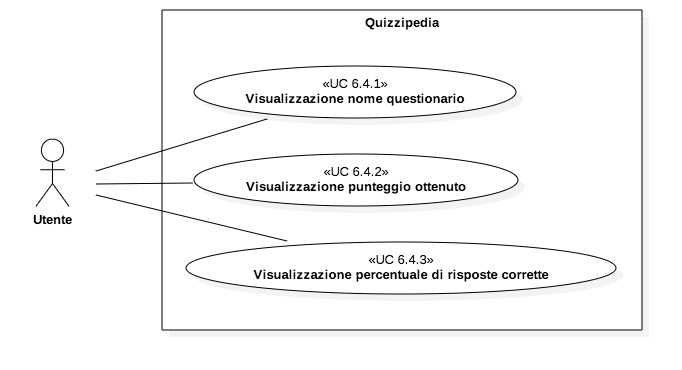
\includegraphics[scale=0.6]{../immagini/UC6_5.png}
\caption{Valutazione questionario}
\end{figure}
\ \\
\textbf{Attori:} \textit{utente}
\\ \\
\textbf{Descrizione:} caso d'uso che descrive la valutazione di un questionario consegnato.\\
\\
\textbf{Precondizioni:} l'utente ha compilato e consegnato un questionario.\\
\\
\textbf{Postcondizioni:} l'utente visualizza la valutazione del questionario.\\
\\
\textbf{Scenario:} il sistema valuta il questionario e visualizza i risultati.\\


\subsubsubsection{UC 6.5.1 - Visualizzazione nome questionario}

\textbf{Attori:} \textit{utente}
\\ \\
\textbf{Descrizione:} caso d'uso che descrive la visualizzazione del nome del questionario valutato.\\
\\
\textbf{Precondizioni:} l'utente ha consegnato un questionario che è stato valutato dal sistema.\\
\\
\textbf{Postcondizioni:} il sistema visualizza il nome del questionario valutato.\\
\\
\textbf{Scenario:} l’utente visualizza il nome del questionario valutato.\\


\subsubsubsection{UC 6.5.2 - Visualizzazione punteggio ottenuto}

\textbf{Attori:} \textit{utente}
\\ \\
\textbf{Descrizione:} caso d'uso che descrive la visualizzazione del punteggio ottenuto nel questionario valutato.\\
\\
\textbf{Precondizioni:} l'utente ha consegnato un questionario che è stato valutato dal sistema.\\
\\
\textbf{Postcondizioni:} il sistema visualizza il punteggio ottenuto nel questionario valutato.\\
\\
\textbf{Scenario:} l’utente visualizza il punteggio ottenuto nel questionario valutato.\\


\subsubsubsection{UC 6.5.3 - Visualizzazione percentuale risposte corrette}

\textbf{Attori:} \textit{utente}
\\ \\
\textbf{Descrizione:} caso d'uso che descrive la visualizzazione della percentuale risposte corrette nel questionario valutato.\\
\\
\textbf{Precondizioni:} l'utente ha consegnato un questionario che è stato valutato dal sistema.\\
\\
\textbf{Postcondizioni:} il sistema visualizza la percentuale risposte corrette nel questionario valutato.\\
\\
\textbf{Scenario:} l’utente visualizza la percentuale risposte corrette nel questionario valutato.\\


\newpage
\subsection{UC 7 - Creazione domanda}

\begin{figure}[h!]
\centering
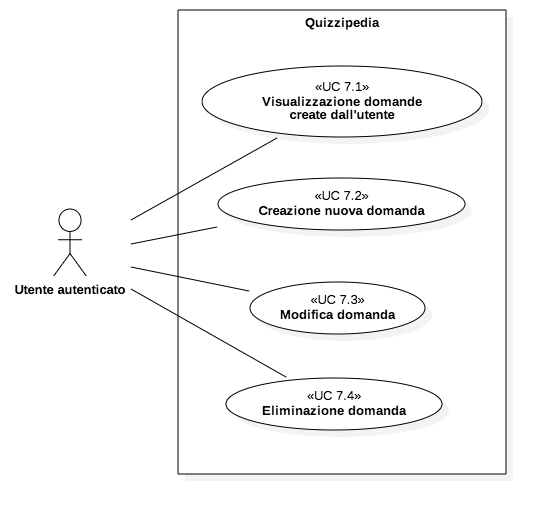
\includegraphics[scale=0.6]{../immagini/UC7.png}
\caption{Creazione domanda}
\end{figure}
\ \\
\textbf{Attori:} \textit{utente autenticato}
\\ \\
\textbf{Descrizione:} caso d'uso che descrive la creazione di una nuova domanda.\\
\\
\textbf{Precondizioni:} l'utente può creare una domanda.\\
\\
\textbf{Postcondizioni:} l’utente ha creato una nuova domanda.\\
\\
\textbf{Scenario:} l’utente inserisce i dati della domanda (UC 7.1, UC 7.2) e li invia al sistema che memorizza la nuova domanda (UC 7.3). Se all'invio alcuni dati essenziali mancano viene visualizzato un messaggio di errore (UC 7.4).\\


\subsubsection{UC 7.1 - Inserimento categorie domanda}

\textbf{Attori:} \textit{utente autenticato}
\\ \\
\textbf{Descrizione:} caso d'uso che descrive l'inserimento delle categorie della domanda.\\
\\
\textbf{Precondizioni:} il sistema permette l'inserimento di una o più categorie.\\
\\
\textbf{Postcondizioni:} l’utente ha inserito almeno una categoria.\\
\\
\textbf{Scenario:} l’utente inserisce una o più categorie nell'apposito campo.\\


\subsubsection{UC 7.2 - Inserimento QML domanda}

\textbf{Attori:} \textit{utente autenticato}
\\ \\
\textbf{Descrizione:} caso d'uso che descrive l'inserimento del codice QML che descrive la domanda.\\
\\
\textbf{Precondizioni:} il sistema permette l'inserimento di codice QML.\\
\\
\textbf{Postcondizioni:} l’utente ha inserito il codice QML che descrive la domanda.\\
\\
\textbf{Scenario:} l’utente inserisce il codice QML che descrive la domanda nell'apposita area di testo.\\


\subsubsection{UC 7.3 - Invio dati domanda}

\textbf{Attori:} \textit{utente autenticato}
\\ \\
\textbf{Descrizione:} caso d'uso che descrive l'invio dei dati della nuova domanda.\\
\\
\textbf{Precondizioni:} l'utente ha inserito i dati della domanda.\\
\\
\textbf{Postcondizioni:} l’utente ha inviato i dati della domanda e il sistema l'ha memorizzata nel database.\\
\\
\textbf{Scenario:} l’utente invia i dati della domanda. Il sistema memorizza nel database la nuova domanda.\\
\\
\textbf{Extension points:} 
\begin{itemize}
	\item \textbf{Dati domanda mancanti:} almeno un dato richiesto non è stato inserito dall'utente, viene visualizzato un messaggio di errore (UC 7.4)
\end{itemize}


\newpage
\subsection{UC 8 - Creazione questionario}

\begin{figure}[h!]
\centering
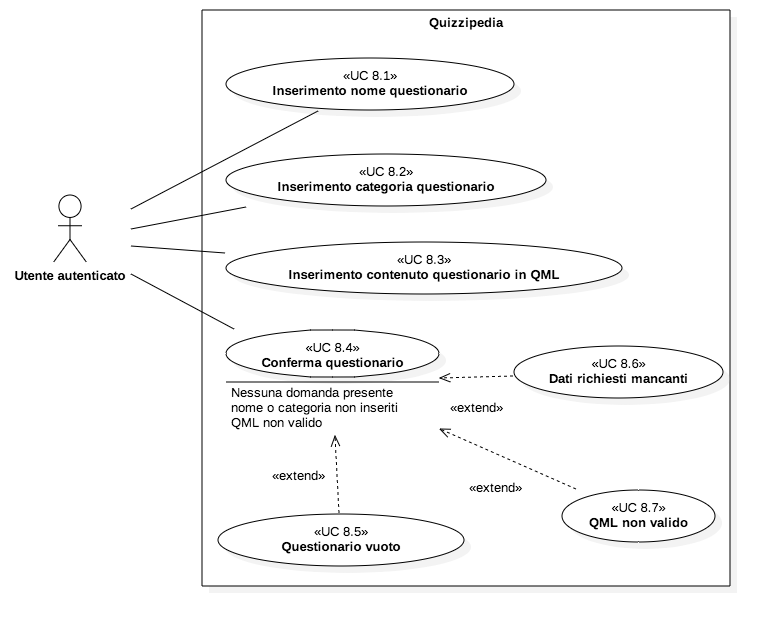
\includegraphics[scale=0.6]{../immagini/UC8.png}
\caption{Creazione questionario}
\end{figure}
\ \\
\textbf{Attori:} \textit{utente autenticato}
\\ \\
\textbf{Descrizione:} caso d'uso che descrive la creazione di un nuovo questionario.\\
\\
\textbf{Precondizioni:} l'utente può creare un questionario.\\
\\
\textbf{Postcondizioni:} l’utente ha creato un nuovo questionario.\\
\\
\textbf{Scenario:} l’utente inserisce i dati del questionario (UC 8.1, UC 8.2, UC 8.3) e li invia al sistema che memorizza il nuovo questionario (UC 8.4). Se all'invio il questionario risulta vuoto viene visualizzato un messaggio di errore (UC 8.5). Se all'invio alcuni dati essenziali mancano viene visualizzato un messaggio di errore (UC 8.6).\\


\subsubsection{UC 8.1 - Inserimento nome questionario}

\textbf{Attori:} \textit{utente autenticato}
\\ \\
\textbf{Descrizione:} caso d'uso che descrive l'inserimento del nome del questionario.\\
\\
\textbf{Precondizioni:} il sistema permette l'inserimento di un nome.\\
\\
\textbf{Postcondizioni:} l’utente ha inserito il nome del questionario.\\
\\
\textbf{Scenario:} l’utente inserisce il nome del questionario nell'apposito campo.\\


\subsubsection{UC 8.2 - Inserimento categoria questionario}

\textbf{Attori:} \textit{utente autenticato}
\\ \\
\textbf{Descrizione:} caso d'uso che descrive l'inserimento della categoria del questionario.\\
\\
\textbf{Precondizioni:} il sistema permette l'inserimento di una categoria.\\
\\
\textbf{Postcondizioni:} l’utente ha inserito la categoria del questionario.\\
\\
\textbf{Scenario:} l’utente inserisce la categoria del questionario nell'apposito campo.\\


\subsubsection{UC 8.3 - Inserimento QML questionario}

\textbf{Attori:} \textit{utente autenticato}
\\ \\
\textbf{Descrizione:} caso d'uso che descrive l'inserimento del codice QML che descrive il questionario.\\
\\
\textbf{Precondizioni:} il sistema permette l'inserimento di codice QML.\\
\\
\textbf{Postcondizioni:} l’utente ha inserito il codice QML che descrive il questionario.\\
\\
\textbf{Scenario:} l’utente inserisce il codice QML che descrive il questionario nell'apposita area di testo.\\


\subsubsection{UC 8.4 - Conferma questionario}

\textbf{Attori:} \textit{utente autenticato}
\\ \\
\textbf{Descrizione:} caso d'uso che descrive l'invio dei dati del nuovo questionario.\\
\\
\textbf{Precondizioni:} l'utente ha inserito i dati del questionario.\\
\\
\textbf{Postcondizioni:} l’utente ha inviato i dati del questionario e il sistema l'ha memorizzato nel database.\\
\\
\textbf{Scenario:} l’utente invia i dati del questionario. Il sistema memorizza nel database il nuovo questionario.\\
\\
\textbf{Extension points:} 
\begin{itemize}
	\item \textbf{Questionario vuoto:} l'utente non ha inserito nessuna domanda nel questionario, viene visualizzato un messaggio di errore (UC 8.5)
	\item \textbf{Dati richiesti mancanti:} il nome e/o la categoria del questionario non sono stati inseriti dall'utente, viene visualizzato un messaggio di errore (UC 8.6)
\end{itemize}


\subsection{UC 9 - Logout}

\textbf{Attori:} \textit{utente autenticato}
\\ \\
\textbf{Descrizione:} caso d'uso che descrive il logout dell'utente.\\
\\
\textbf{Precondizioni:} il sistema permette il logout.\\
\\
\textbf{Postcondizioni:} l’utente non è più autenticato.\\
\\
\textbf{Scenario:} l’utente clicca su logout. Il sistema non riconosce più come autenticato l'utente.\\

	
	
	
	\newpage
	\section{Requisiti}
		Di seguito vengono elencati i requisiti emersi in fase di analisi del capitolato e del problema.\\
		I requisiti sono presentati in maniera gerarchica affinché i sotto-requisiti specifichino ulteriori informazioni e dettagli rispetto al loro genitore.\\
		Per avere una migliore organizzazione dei requisiti questi vengono suddivisi in funzionali (F), QML (QML), di qualità (Q) e vincoli di sistema imposti dal capitolato (V).\\
		Dopo la categoria ogni codice identificativo è completato da un numero che mostra anche il livello e l'appartenenza della gerarchia sopra descritta.\\
		\subsection{Requisiti funzionali}
			\begin{longtable}{p{0.2\columnwidth}p{0.8\textwidth}}
			\caption{Requisiti funzionali} \\

ID & Descrizione \\
\midrule
\endfirsthead

ID & Descrizione \\
\midrule
\endhead

\multicolumn{2}{c}{\footnotesize\itshape\tablename~\thetable: Requisiti funzionali}
\endfoot

\multicolumn{2}{c}{\footnotesize\itshape\tablename~\thetable: Requisiti funzionali}
\endlastfoot
			
F 1 & Il sistema deve fornire la possibilità ad un utente non autenticato di registrarsi\\
\midrule
F 1.1 & La sezione dedicata alla registrazione deve permettere l'inserimento dei dati necessari\\
\midrule
F 1.1.1 & La sezione dedicata alla registrazione deve permettere l'inserimento di una e-mail\\
\midrule
F 1.1.2 & La sezione dedicata alla registrazione deve permettere l'inserimento di una password\\
\midrule
F 1.2 & La sezione dedicata alla registrazione deve permettere l'invio dei dati inseriti\\
\midrule
F 1.2.1 & Prima di inviare i dati viene effettuato un controllo su di essi\\
\midrule
F 1.2.1.1 & Se i dati non risultano corretti viene visualizzato un messaggio di errore\\
\midrule
F 1.2.1.2 & Se i dati non risultano corretti non vengono inviati\\
\midrule
F 1.2.2 & Quando dei dati corretti vengono inviati il sistema memorizza un nuovo account con essi\\
\midrule
F 1.2.3 & Quando viene creato un nuovo account con la procedura di registrazione viene automaticamente effettuato il login con quell'account\\
\midrule
F 2 & Il sistema deve fornire la possibilità ad un utente non autenticato di autenticarsi\\
\midrule
F 2.1 & La sezione dedicata all'autenticazione deve permettere l'inserimento dei dati necessari\\
\midrule
F 2.1.1 & La sezione dedicata all'autenticazione deve permettere l'inserimento di una e-mail\\
\midrule
F 2.1.2 & La sezione dedicata all'autenticazione deve permettere l'inserimento di una password\\
\midrule
F 2.2 & La sezione dedicata all'autenticazione deve fornire l'opzione ricordami\\
\midrule
F 2.3 & La sezione dedicata all'autenticazione deve permettere l'invio dei dati inseriti\\
\midrule
F 2.3.1 & Prima di inviare i dati viene effettuato un controllo su di essi\\
\midrule
F 2.3.1.1 & Se la combinazione e-mail/password non è registrata viene visualizzato un messaggio di errore\\
\midrule
F 2.3.2 & Se la combinazione e-mail/password è registrata l'utente viene autenticato\\
\midrule
F 2.3.3 & Se la combinazione e-mail/password è registrata e l'opzione ricordami è stata selezionata viene memorizzata l'e-mail con un cookie\\
\midrule
F 2.4 & La sezione dedicata all'autenticazione deve fornire una procedura di recupero password\\
\midrule
F 2.4.1 & La procedura di recupero password deve permettere l'inserimento della e-mail\\
\midrule
F 2.4.2 & La procedura di recupero password deve effettuare un controllo sulla e-mail inserita\\
\midrule
F 2.4.2.1 & Se la e-mail non risulta registrata viene visualizzato un messaggio di errore\\
\midrule
F 2.4.2.2 & Se la e-mail non risulta registrata non viene mandata una mail a quell'indirizzo\\
\midrule
F 2.4.3 & La procedura di recupero password deve mandare una mail all'indirizzo inserito con la password dimenticata\\
\midrule
F 3 & Il sistema deve fornire una sezione con un elenco delle categorie di questionari presenti nel database\\
\midrule
F 3.1 & Quando l'utente seleziona una categoria viene visualizzato un elenco dei questionari della categoria scelta presenti nel database\\
\midrule
F 4 & L'utente può scegliere un qualsiasi questionario cliccandoci sopra per compilarlo\\
\midrule
F 4.1 & Durante la compilazione del questionario un utente può navigare liberamente tra le domande che lo compongono\\
\midrule
F 4.2 & L'utente può rispondere alle domande\\
\midrule
F 4.2.1 & Se la domanda è di tipo vero o falso vengono fornite due opzioni: Vero e Falso\\
\midrule
F 4.2.2 & Se la domanda è a risposta multipla vengono fornita la lista di possibili risposte\\
\midrule
F 4.2.3 & Se la domanda richiede una risposta inserita dall'utente allora viene fornito un campo per l'inserimento della risposta\\
\midrule
F 4.3 & L'utente può cambiare la risposta di una domanda in qualsiasi momento prima della consegna del questionario\\
\midrule
F 4.4 & Le domande possono essere compilate in un ordine qualsiasi\\
\midrule
F 4.5 & L'utente può consegnare il questionario\\
\midrule
F 4.5.1 & Se alla consegna una o più domande non sono state compilate il sistema avverte l'utente di ciò\\
\midrule
F 4.5.2 & Quando un questionario viene confermato e consegnato vengono memorizzate nel database le risposte date\\
\midrule
F 4.5.3 & Quando un questionario viene confermato e consegnato viene valutato dal sistema\\
\midrule
F 4.5.3.1 & La valutazione del questionario viene visualizzata all'utente\\
\midrule
F 5 & Il sistema deve fornire la possibilità ad un utente autenticato di creare una nuova domanda\\
\midrule
F 5.1 & La sezione dedicata alla creazione di una domanda deve permettere l'inserimento dei dati necessari\\
\midrule
F 5.1.1 & La sezione dedicata alla creazione di una domanda deve permettere la scelta di una o più categorie\\
\midrule
F 5.1.2 & La sezione dedicata alla creazione di una domanda deve permettere l'inserimento del testo della domanda\\
\midrule
F 5.1.3 & La sezione dedicata alla creazione di una domanda deve permettere la scelta della tipologia della domanda\\
\midrule
F 5.1.3.1 & Nel caso in cui la tipologia scelta sia a risposta multipla la sezione dedicata alla creazione di una domanda deve permettere l'inserimento di due o più possibili risposte\\
\midrule
F 5.1.4 & La sezione dedicata alla creazione di una domanda deve permettere l'inserimento della risposta corretta\\
\midrule
F 5.2 & La sezione dedicata alla creazione di una domanda deve permettere l'invio dei dati inseriti\\
\midrule
F 5.2.1 & Prima di inviare i dati viene effettuato un controllo su di essi\\
\midrule
F 5.2.1.1 & Se i dati obbligatori non risultano inseriti viene visualizzato un messaggio di errore\\
\midrule
F 5.2.1.2 & Se i dati obbligatori non risultano inseriti nessun dato viene inviato\\
\midrule
F 5.2.2 & Quando dei dati che superano i controlli vengono inviati viene creata una nuova domanda con essi e inserita nel database\\
\midrule
F 5.2.2.1 & Se la creazione di una nuova domanda va a buon fine il sistema avvisa l'utente\\
\midrule
F 5.2.2.2 & Se la creazione di una nuova domanda non va a buon fine il sistema visualizza un messaggio di errore\\
\midrule
F 6 & Il sistema deve fornire la possibilità ad un utente autenticato di creare un nuovo questionario\\
\midrule
F 6.1 & La sezione dedicata alla creazione di un questionario deve permettere l'inserimento dei dati necessari\\
\midrule
F 6.1.1 & La sezione dedicata alla creazione di un questionario deve permettere l'inserimento del nome del questionario\\
\midrule
F 6.1.2 & La sezione dedicata alla creazione di un questionario deve permettere la scelta della categoria del questionario\\
\midrule
F 6.1.2.1 & Una volta scelta la categoria la sezione dedicata alla creazione di un questionario deve visualizzare la lista delle domande di quella categoria presenti nel database non ancora inserite nel questionario\\
\midrule
F 6.1.3 & La sezione dedicata alla creazione di un questionario deve permettere l'aggiunta di una domanda della lista di F 6.1.2.1 nel questionario\\
\midrule
F 6.1.4 & La sezione dedicata alla creazione di un questionario deve visualizzare la lista di domande già inserite nel questionario\\
\midrule
F 6.2 & La sezione dedicata alla creazione di una nuova domanda deve permettere l'invio dei dati inseriti\\
\midrule
F 6.2.1 & Prima di inviare i dati viene effettuato un controllo su di essi\\
\midrule
F 6.2.1.1 & Se i dati obbligatori non risultano inseriti viene visualizzato un messaggio di errore\\
\midrule
F 6.2.1.2 & Se i dati obbligatori non risultano inseriti nessun dato viene inviato\\
\midrule
F 6.2.2 & Quando dei dati che superano i controlli vengono inviati viene creato un nuovo questionario con essi e inserito nel database\\
\midrule
F 6.2.2.1 & Se la creazione di un nuovo questionario va a buon fine il sistema avvisa l'utente\\
\midrule
F 6.2.2.2 & Se la creazione di un nuovo questionario non va a buon fine il sistema visualizza un messaggio di errore\\
\midrule
F 7 & Il sistema deve fornire la possibilità ad un utente autenticato di uscire facendo il logout\\
			
			\end{longtable}
		\subsection{Requisiti QML}
			\begin{longtable}{p{0.2\columnwidth}p{0.8\textwidth}}
			\caption{Requisiti QML} \\

ID & Descrizione \\
\midrule
\endfirsthead

ID & Descrizione \\
\midrule
\endhead

\multicolumn{2}{c}{\footnotesize\itshape\tablename~\thetable: Requisiti QML}
\endfoot

\multicolumn{2}{c}{\footnotesize\itshape\tablename~\thetable: Requisiti QML}
\endlastfoot
			
QML 1 & QML definisce domande\\
\midrule
QML 1.1 & Una domanda è formata dal testo del quesito e da una o più risposte\\
\midrule
QML 1.2 & Una domanda deve avere almeno una risposta esatta\\
\midrule
QML 1.3 & Una domanda può avere una lista di possibili risposte\\
\midrule
QML 1.4 & Una domanda deve appartenere ad una o più categorie\\
\midrule
QML 1.5 & Una domanda deve avere una tipologia definita da QML\\
\midrule
QML 1.5.1 & QML definisce domande di tipo vero o falso\\
\midrule
QML 1.5.2 & QML definisce domande a scelta multipla\\
\midrule
QML 1.5.3 & QML definisce domande a risposta testuale\\
\midrule
QML 2 & QML definisce questionari\\
\midrule
QML 2.1 & Un questionario è formato da una lista di domande\\
\midrule
QML 2.2 & Un questionario appartiene ad una sola categoria\\
\midrule
QML 3 & QML gestisce immagini all'interno di domande e risposte\\
			
			\end{longtable}
		\subsection{Requisiti di qualità}
			\begin{longtable}{p{0.2\columnwidth}p{0.8\textwidth}}
			\caption{Requisiti di qualità} \\

ID & Descrizione \\
\midrule
\endfirsthead

ID & Descrizione \\
\midrule
\endhead

\multicolumn{2}{c}{\footnotesize\itshape\tablename~\thetable: Requisiti di qualità}
\endfoot

\multicolumn{2}{c}{\footnotesize\itshape\tablename~\thetable: Requisiti di qualità}
\endlastfoot
			
Q 1 & Le pagine web dell'applicazione avranno una netta separazione tra struttura, stile e contenuto\\
\midrule
Q 1.1 & L'applicazione permette facilmente la modifica della struttura senza intaccare il resto\\
\midrule
Q 1.2 & L'applicazione permette facilmente la modifica dello stile senza intaccare il resto\\
\midrule
Q 1.3 & L'applicazione permette facilmente la modifica dei contenuti senza intaccare il resto\\
\midrule
Q 2 & Il codice HTML passa il test di validazione del W3C\\
\midrule
Q 3 & Il codice CSS passa il test di validazione del W3C\\
			
			\end{longtable}
		\subsection{Vincoli di sistema}
			\begin{longtable}{p{0.2\columnwidth}p{0.8\textwidth}}
			\caption{Vincoli di sistema} \\

ID & Descrizione \\
\midrule
\endfirsthead

ID & Descrizione \\
\midrule
\endhead

\multicolumn{2}{c}{\footnotesize\itshape\tablename~\thetable: Vincoli di sistema}
\endfoot

\multicolumn{2}{c}{\footnotesize\itshape\tablename~\thetable: Vincoli di sistema}
\endlastfoot
			
V 1 & Il sistema deve essere realizzato con tecnologie web\\
\midrule
V 2 & Il sistema deve essere utilizzabile attraverso un browser\\
\midrule
V 2.1 & L'interfaccia utente deve essere fruibile via desktop, tablet e smartphone\\
\midrule
V 2.2 & L'interfaccia utente deve essere strutturata con html 5\\
\midrule
V 2.3 & Lo stile dell'interfaccia utente deve essere realizzato tramite fogli di stile css 3\\
\midrule
V 2.4 & La parte attiva dell'interfaccia utente deve essere gestita utilizzando javascript\\
\midrule
V 3 & Domande e questionari vengono memorizzati in QML\\
\midrule
V 4 & La parte server viene realizzata in javascript con server Node.js\\
			
			\end{longtable}
	
	\newpage
	\section{Mappature}
		\subsection{Mappatura casi d'uso - requisiti}
			\begin{longtable}{p{0.5\columnwidth}p{0.5\textwidth}}
			\caption{Mappatura casi d'uso - requisiti} \\

Caso d'uso & Requisito \\
\midrule
\endfirsthead

Caso d'uso & Requisito \\
\midrule
\endhead

\multicolumn{2}{c}{\footnotesize\itshape\tablename~\thetable: Mappatura casi d'uso - requisiti}
\endfoot

\multicolumn{2}{c}{\footnotesize\itshape\tablename~\thetable: Mappatura casi d'uso - requisiti}
\endlastfoot
			
UC 1 & F 1, F 2, F 3, F 3.1, F 4, F 5, F 6, F 7\\
\midrule
UC 1.1 & F 2\\
\midrule
UC 1.1.1 & F 2.1.1\\
\midrule
UC 1.1.2 & F 2.1.2\\
\midrule
UC 1.1.3 & F 2.2\\
\midrule
UC 1.1.4 & F 2.4\\
\midrule
UC 1.1.4.1 & F 2.4.1\\
\midrule
UC 1.1.4.2 & F 2.4.3\\
\midrule
UC 1.1.5 & F 2.1.3\\
\midrule
UC 1.2 & F 1\\
\midrule
UC 1.2.1 & F 1.1.1\\
\midrule
UC 1.2.2 & F 1.1.2\\
\midrule
UC 1.2.3 & F 1.2\\
\midrule
UC 1.3 & F 3\\
\midrule
UC 1.4 & F 3.1\\
\midrule
UC 1.5 & F 4\\
\midrule
UC 1.6 & F 4.2, 4.5\\
\midrule
UC 1.6.1 & F 4.2\\
\midrule
UC 1.6.2 & F 4.5\\
\midrule
UC 1.6.3 & F 4.5.3\\
\midrule
UC 1.6.4 & F 4.5.3.1\\
\midrule
UC 1.7 & F 5\\
\midrule
UC 1.7.1 & F 5.1.1\\
\midrule
UC 1.7.2 & F 5.1.2\\
\midrule
UC 1.7.3 & F 5.1.3\\
\midrule
UC 1.7.5 & F 5.1.4\\
\midrule
UC 1.7.6 & F 5.2\\
\midrule
UC 1.8 & F 6\\
\midrule
UC 1.8.1 & F 6.1.1\\
\midrule
UC 1.8.2 & F 6.1.2\\
\midrule
UC 1.8.3 & F 6.1.3\\
\midrule
UC 1.8.4 & F 6.2\\
\midrule
UC 1.9 & F 7\\

			
			\end{longtable}

		\subsection{Mappatura requisiti - casi d'uso}
			\begin{longtable}{p{0.5\columnwidth}p{0.5\textwidth}}
			\caption{Mappatura requisiti - casi d'uso} \\

Requisito & Caso d'uso \\
\midrule
\endfirsthead

Requisito & Caso d'uso \\
\midrule
\endhead

\multicolumn{2}{c}{\footnotesize\itshape\tablename~\thetable: Mappatura requisiti - casi d'uso}
\endfoot

\multicolumn{2}{c}{\footnotesize\itshape\tablename~\thetable: Mappatura requisiti - casi d'uso}
\endlastfoot
			
F 1 & UC 2\\
\midrule
F 1.1 & UC 1.2.1, UC 1.2.2\\
\midrule
F 1.1.1 & UC 1.2.1\\
\midrule
F 1.1.2 & UC 1.2.2\\
\midrule
F 1.2 & UC 1.2.3\\
\midrule
F 1.2.1 & UC 1.2.3\\
\midrule
F 1.2.1.1 & UC 1.2.4\\
\midrule
F 1.2.1.2 & UC 1.2.4\\
\midrule
F 1.2.2 & UC 1.2.3\\
\midrule
F 1.2.3 & UC 1.2.3\\
\midrule
F 2 & UC 1.1\\
\midrule
F 2.1 & UC 1.1.1, UC 1.1.2\\
\midrule
F 2.1.1 & UC 1.1.1\\
\midrule
F 2.1.2 & UC 1.1.2\\
\midrule
F 2.2 & UC 1.1.3\\
\midrule
F 2.3 & UC 1.1.5\\
\midrule
F 2.3.1 & UC 1.1.5\\
\midrule
F 2.3.1.1 & UC 1.1.6\\
\midrule
F 2.3.2 & UC 1.1.5\\
\midrule
F 2.3.3 & UC 1.1.7\\
\midrule
F 2.4 & UC 1.1.4\\
\midrule
F 2.4.1 & UC 1.1.4.1\\
\midrule
F 2.4.2 & UC 1.1.4.2\\
\midrule
F 2.4.2.1 & UC 1.1.4.3\\
\midrule
F 2.4.2.2 & UC 1.1.4.3\\
\midrule
F 2.4.3 & UC 1.1.4.2\\
\midrule
F 3 & UC 1.3\\
\midrule
F 3.1 & UC 1.4\\
\midrule
F 4 & UC 1.5\\
\midrule
F 4.1 & Non mappabile\\
\midrule
F 4.2 & UC 1.6.1\\
\midrule
F 4.2.1 & UC 1.6.1\\
\midrule
F 4.2.2 & UC 1.6.1\\
\midrule
F 4.2.3 & UC 1.6.1\\
\midrule
F 4.3 & UC 1.6.1\\
\midrule
F 4.4 & Non mappabile\\
\midrule
F 4.5 & UC 1.6.2\\
\midrule
F 4.5.1 & UC 1.6.5\\
\midrule
F 4.5.2 & UC 1.6.3\\
\midrule
F 4.5.3 & UC 1.6.3\\
\midrule
F 4.5.3.1 & UC 1.6.4\\
\midrule
F 5 & UC 1.7\\
\midrule
F 5.1 & UC 1.7.1, UC 1.7.2, UC 1.7.3, UC 1.7.4, UC 1.7.5\\
\midrule
F 5.1.1 & UC 1.7.1\\
\midrule
F 5.1.2 & UC 1.7.2\\
\midrule
F 5.1.3 & UC 1.7.3\\
\midrule
F 5.1.3.1 & UC 1.7.4\\
\midrule
F 5.1.4 & UC 1.7.5\\
\midrule
F 5.2 & UC 1.7.6\\
\midrule
F 5.2.1 & UC 1.7.6\\
\midrule
F 5.2.1.1 & UC 1.7.7\\
\midrule
F 5.2.1.2 & UC 1.7.7\\
\midrule
F 5.2.2 & UC 1.7.6\\
\midrule
F 5.2.2.1 & UC 1.7.6\\
\midrule
F 5.2.2.2 & UC 1.7.7\\
\midrule
F 6 & UC 1.8\\
\midrule
F 6.1 & UC 1.8.1, UC 1.8.2, UC 1.8.3\\
\midrule
F 6.1.1 & UC 1.8.1\\
\midrule
F 6.1.2 & UC 1.8.2\\
\midrule
F 6.1.2.1 & UC 1.8.2\\
\midrule
F 6.1.3 & UC 1.8.3\\
\midrule
F 6.1.4 & Non mappabile\\
\midrule
F 6.2 & UC 1.8.4\\
\midrule
F 6.2.1 & UC 1.8.4\\
\midrule
F 6.2.1.1 & UC 1.8.5\\
\midrule
F 6.2.1.2 & UC 1.8.5\\
\midrule
F 6.2.2 & UC 1.8.4\\
\midrule
F 6.2.2.1 & UC 1.8.4\\
\midrule
F 6.2.2.2 & UC 1.8.5\\
\midrule
F 7 & UC 1.9\\
\midrule

			
			\end{longtable}
			
\end{document}